\let\negmedspace\undefined
\let\negthickspace\undefined
\documentclass[journal]{IEEEtran}
\usepackage[a5paper, margin=10mm, onecolumn]{geometry}
%\usepackage{lmodern} % Ensure lmodern is loaded for pdflatex
\usepackage{tfrupee} % Include tfrupee package

\setlength{\headheight}{1cm} % Set the height of the header box
\setlength{\headsep}{0mm}     % Set the distance between the header box and the top of the text

\usepackage{gvv-book}
\usepackage{gvv}
\usepackage{cite}
\usepackage{amsmath,amssymb,amsfonts,amsthm}
\usepackage{algorithmic}
\usepackage{graphicx}
\usepackage{textcomp}
\usepackage{xcolor}
\usepackage{txfonts}
\usepackage{listings}
\usepackage{enumitem}
\usepackage{mathtools}
\usepackage{gensymb}
\usepackage{comment}
\usepackage[breaklinks=true]{hyperref}
\usepackage{tkz-euclide} 
\usepackage{listings}
% \usepackage{gvv}                                        
\def\inputGnumericTable{}                                 
\usepackage[latin1]{inputenc}                                
\usepackage{color}                                            
\usepackage{array}                                            
\usepackage{longtable}                                       
\usepackage{calc}                                             
\usepackage{multirow}                                         
\usepackage{hhline}                                           
\usepackage{ifthen}                                           
\usepackage{lscape}
\usepackage{circuitikz}
\tikzstyle{block} = [rectangle, draw, fill=blue!20, 
    text width=4em, text centered, rounded corners, minimum height=3em]
\tikzstyle{sum} = [draw, fill=blue!10, circle, minimum size=1cm, node distance=1.5cm]
\tikzstyle{input} = [coordinate]
\tikzstyle{output} = [coordinate]
\begin{document}
\textbf{Question:}  
Let $\vec a = 4\hat\imath+5\hat\jmath-\hat k$, $\vec b=\hat\imath-4\hat\jmath+5\hat k$, $\vec c=3\hat\imath+\hat\jmath-\hat k$.  
Find $\vec d$ perpendicular to both $\vec b$ and $\vec c$ and satisfying $\vec d\cdot\vec a=21$.

\medskip

\textbf{Solution:}  

Write vectors as column matrices:
\[
\vec a=\begin{pmatrix}4\\5\\-1\end{pmatrix},\quad
\vec b=\begin{pmatrix}1\\-4\\5\end{pmatrix},\quad
\vec c=\begin{pmatrix}3\\1\\-1\end{pmatrix}.
\]

Since $\vec d$ is perpendicular to both $\vec b$ and $\vec c$,  
\[
\vec d = \lambda(\vec b\times \vec c).
\]

Compute the cross product:
\[
\vec b\times \vec c =\begin{pmatrix}
(-4)(-1)-5(1)\\[6pt]
-\big(1(-1)-5(3)\big)\\[6pt]
1(1)-(-4)(3)
\end{pmatrix}
=
\begin{pmatrix}-1\\16\\13\end{pmatrix}.
\]

Thus
\[
\vec d = \lambda \begin{pmatrix}-1\\16\\13\end{pmatrix}.
\]

Now apply the condition $\vec d\cdot \vec a = 21$:
\[
\vec d \cdot \vec a 
= \lambda \begin{pmatrix}-1 & 16 & 13\end{pmatrix}
\begin{pmatrix}4\\5\\-1\end{pmatrix}.
\]

\[
= \lambda(-4+80-13)=\lambda(63).
\]

So
\[
\lambda(63)=21 \quad\Rightarrow\quad \lambda=\tfrac{1}{3}.
\]

Hence
\[
\vec d = \tfrac{1}{3}\begin{pmatrix}-1\\16\\13\end{pmatrix}
= -\tfrac{1}{3}\hat\imath + \tfrac{16}{3}\hat\jmath + \tfrac{13}{3}\hat k.
\]

\[
\boxed{\vec d = -\tfrac{1}{3}\hat\imath + \tfrac{16}{3}\hat\jmath + \tfrac{13}{3}\hat k}
\]
\begin{figure}
    \centering
    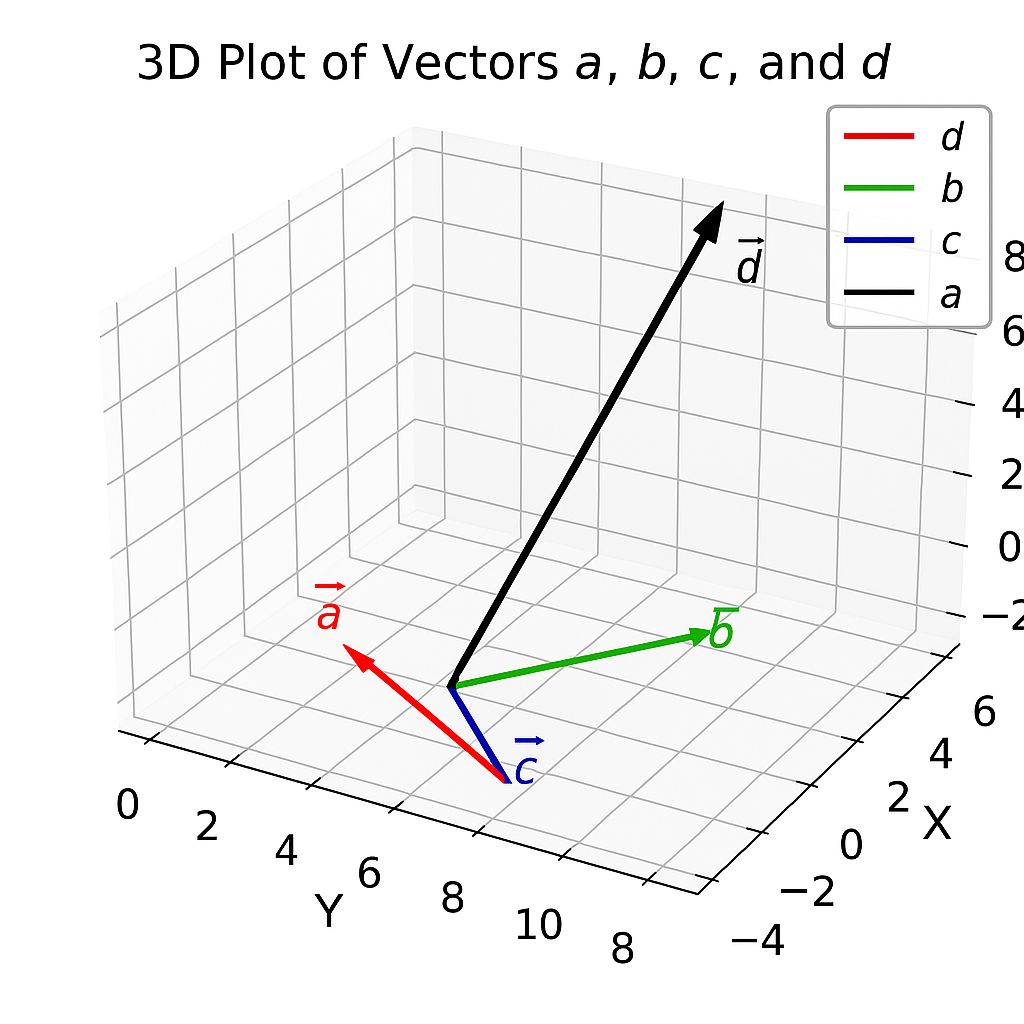
\includegraphics[width=0.5\linewidth]{figs/plot.png}
    \caption{plot}
    \label{fig:placeholder}
\end{figure}
\end{document}